\documentclass[
	english,
        solution=true
	]{tudaexercise}

\usepackage[main=english, ngerman]{babel}
\usepackage[babel]{csquotes}

\usepackage{amstext}
\usepackage{amsmath}
\usepackage{amssymb}
\usepackage{graphicx}
\usepackage{setspace}
\usepackage{multicol}
\usepackage{mathtools}
\usepackage{dsfont}
\usepackage{units}
\usepackage{subfigure}
\usepackage{color}
\usepackage{booktabs}
\usepackage{fancyref}
\usepackage{listings}
\usepackage{mathrsfs}
\usepackage{physics}
\usepackage{gauss}
\usepackage{bm}
\usepackage{multirow}
\usepackage{pgfplots}
\usepackage{pgfplotstable}
\usetikzlibrary{patterns}


\let\file\texttt
\let\code\texttt
\let\pck\textsf
\let\cls\textsf
\let\tbs\textbackslash

\ConfigureHeadline{
	headline={title}
}

%compatbilitx
\let\unit\relax

% math commands
\newcommand{\R}{\mathbb{R}}
\DeclareMathOperator*{\argmax}{arg\,max}
\DeclareMathOperator*{\argmin}{arg\,min}

\begin{document}

\author{Prof. Marcus Rohrbach, Prof. Simone Schaub-Meyer}
\term{Summer Term 2025}

\title[Statistical Machine Learning Exercise 1]{\LARGE Statistical Machine Learning: Exercise 1}
\subtitle{Refresher: Linear Algebra, Probabilities, Bayesian Decision Theory and Risk Minimization\\ Total Possible Points: 85}

\maketitle

\textcolor{red}{\textbf{Publication Date: April 30th, 15:05 PM}}\\
\textcolor{red}{\textbf{Due Date: May 18th, 23:59 PM}}\\

\textbf{Note:} Many of the concepts required for solving this homework will be
introduced in lectures 1, 2, and 3. If you don't know how to do some of these
problems by the time this is released, hold on a bit more for that specific problem. 

Please add your corresponding group number as well as the names of all the members who worked on this assignment to the following section.\\
\textbf{Group 102}\\
\textbf{Members: Lukas Depner, Louis Geiger, Ugurtan Can Cetin}

\begin{task}[points=6]{Machine Learning Introduction}
\begin{subtask}[points=6,title=Model Fitting]
You are given a set of labeled data points, illustrated in the figure below. The striped and solid circles represent the training data, while the triangle is a test point whose true label is solid.

Describe two different classification models, each defined by a linear separation line, that assign different predicted labels to the triangle. One of these models should achieve perfect (100\%) accuracy on the training set.

Briefly explain how the two models differ in terms of training accuracy and in their prediction for the test point, assuming that the true label of the triangle is solid.
\\
\begin{center}
    \begin{tikzpicture}
        % box
        \draw[thick] (0, 0) rectangle (8, 5);
        
        % triangle
        \draw[thick] (3.5, 2.1) -- (4.1, 2.1) -- (3.8, 2.6) -- cycle;
        
        % striped points
        \fill[pattern=north east lines] (1,1) circle[radius=0.25];
        \draw[thick] (1,1) circle[radius=0.25];
    
        \fill[pattern=north east lines] (4.2, 1.2) circle[radius=0.25];
        \draw[thick] (4.2, 1.2) circle[radius=0.25]; 
    
        \fill[pattern=north east lines] (0.7, 2.4) circle[radius=0.25];
        \draw[thick] (0.7, 2.4) circle[radius=0.25];
    
        \fill[pattern=north east lines] (2.3, 1.9) circle[radius=0.25];
        \draw[thick] (2.3, 1.9) circle[radius=0.25];
    
        \fill[pattern=north east lines] (2.2, 3.6) circle[radius=0.25];
        \draw[thick] (2.2, 3.6) circle[radius=0.25];
    
        \fill[pattern=north east lines] (2.8, 4.5) circle[radius=0.25];
        \draw[thick] (2.8, 4.5) circle[radius=0.25]; 
    
        \fill[pattern=north east lines] (0.9, 4.1) circle[radius=0.25];
        \draw[thick] (0.9, 4.1) circle[radius=0.25];
    
        \fill[pattern=north east lines] (3.0, 0.8) circle[radius=0.25];
        \draw[thick] (3.0, 0.8) circle[radius=0.25];
    
        % unstriped points
        \fill[black] (6.4, 1.1) circle (0.25);
        \draw[thick] (6.4, 1.1) circle (0.25);
    
        \fill[black] (4.8, 4.5) circle (0.25);
        \draw[thick] (4.8, 4.5) circle (0.25);
    
        \fill[black] (6.9, 3.5) circle (0.25);
        \draw[thick] (6.9, 3.5) circle (0.25);
    
        \fill[black] (4.1, 3.8) circle (0.25); 
        \draw[thick] (4.1, 3.8) circle (0.25); 
    
        \fill[black] (7.2, 2.5) circle (0.25);
        \draw[thick] (7.2, 2.5) circle (0.25);
    
        \fill[black] (5.7, 3.4) circle (0.25);
        \draw[thick] (5.7, 3.4) circle (0.25);
    
        \fill[black] (5.3, 0.6) circle (0.25);
        \draw[thick] (5.3, 0.6) circle (0.25);
    
        \fill[black] (4.9, 2.3) circle (0.25);
        \draw[thick] (4.9, 2.3) circle (0.25);
    \end{tikzpicture}
\end{center}

\begin{solution}

\begin{center}
    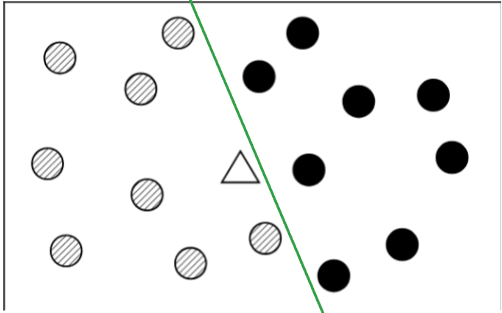
\includegraphics[width=0.5\linewidth]{perfect.png}
\end{center}

The upper classification classifies the triangle as a \textbf{striped circle}. While being $100\%$ correct for the training set, because it separates circle with stripes from the solids, the triangle is wrongly classified, because according to the task description, it should be classified as solid.

\begin{center}
    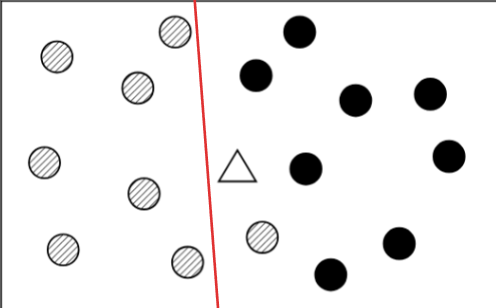
\includegraphics[width=0.5\linewidth]{notperfect.png}
\end{center}

This classification on the other hand, classifies the triangle as a solid, which is the expected label according to the description of the task, but a striped circle is labeled as solid, which means, that the accuracy on the training set is not $100\%$

\textbf{Summary}:
\begin{itemize}
    \item The first model has a training accuracy of 100\%, because the trainins set is separated correctly. But the testpoint (triangle) is classified it as striped instead of solid.
    \item The second model has a lower training accuracy than 100\%, because on training point is labeled wrongly. The testpoint is claasified correctly though.
\end{itemize}

The first model represents overfitting quite well, because it is perfect on the training data, while failing on the test data. The second model represents underfitting, not being completely correct on the training set, but labelling test data correctly.

\end{solution}
\end{subtask}
\end{task}

\newpage

\begin{task}[points=28]{Linear Algebra Refresher}

    \begin{subtask}[points=5,title=Matrix Properties]
A colleague of yours suggests that for matrices, addition and multiplication
works similarly as for scalars, in particular, that the commutative,
distributive and associative properties hold. Are these statements correct?
Prove or disprove them analytically for both operations and all three
properties considering three matrices $ A, B, C$ of size $n\times n$.

\begin{solution}

To proof (or disprove): Addition and multiplication for matrices is commutative, distributive and associative. First we look at each properties by themselves.\\

\begin{itemize}
    \item commutativity:  $\forall a, b \in \R: a+b=b+a$ or $ab=ba$
    \item distributivity: $\forall a, b, c \in \R: a(b+c) = (ab)+(ac)$
    \item associativity: $\forall a, b, c \in \R: a+(b+c)=(a+b)+c$ or $a(bc)=(ab)c$
\end{itemize}

So in the context of matrices we will check each property for multiplication and addition.

\textbf{Addition}

\begin{enumerate}
    \item commutativity: 
    \[ \text{Let } A, B, C \text{ be } n\times n \text{ matrices.}; A=[a_{ij}], B=[b_{ij}], C=[c_{ij}] \text{ and } D=[d_{i_j}] \]
    \[   \text{Let }A+B=C \text{ and } B+A=D. \text{ So out of that, this follows: } c_{ij} = a_{ij} + b_{ij} \text{ and } d_{ij} = b_{ij} + a_{ij}  \]
    \[\text{We have to show: } c_{ij} = d_{ij}\]
    \[d_{ij}=b_{ij}+a_{ij} \,\,\,\,\, | -a_{ij}\]
    \[d_{ij}-a_{ij}=b_{ij}\]
    \[\text{Now we insert that value for }b_{ij} \text{ into the equation for }c_{ij}.\]
    \[c_{ij}=a_{ij}+d_{ij}-a_{ij}\]
    \[c_{ij}=d_{ij} \Rightarrow C=D \Rightarrow \underline{\underline{A+B=B+A}}\]
    % -------------------------------------------
    \item associativity:
    \[\text{Let } A, B, C \text{ be } n \times n \text{ matrices.};  A=[a_{ij}], B=[b_{ij}], C=[c_{ij}] \text{ and } D=[d_{i_j}] \]
    \[A+B=[a_{ij}]+[b_{ij}], \text{ therefore } (A+B)+C = ([a_{ij}] + [b_{ij}])+[c_{ij}].\]
    \[\text{ According to that, this follows: }A+(B+C)=[a_{ij}]+([b_{ij}]+[c_{ij}])\]
    \[\text{On an element level, where the items in addition are numerals, we know that }'+' \text{ is associative.}\]
    \[\text{Thus } (A+B)+C \text{ and } A+(B+C) \text{ are identical. Thus they are equal.}\]
\end{enumerate}
$\Rightarrow$ the addition is commutative and associative with matrices.

\textbf{Multiplication}

\begin{enumerate}
    \item commutativity:
        \[\text{Let } A, B \text{ be }n\times n \text{ matrices, with following values: } A=\begin{pmatrix}
            4 & 1 \\ 3 & 2
        \end{pmatrix}, B=\begin{pmatrix}
            2 & 4 \\1 & 3
        \end{pmatrix}\]
        \[\text{We will assume, that matrix multiplication is commutative.}\]
        \[\text{With given example for $A$ and $B$, $AB$ should equal $BA$}\]
        
        \[AB = \begin{pmatrix}
            4 & 1 \\ 3 & 2
        \end{pmatrix} \begin{pmatrix}
            2 & 4 \\ 1 & 3
        \end{pmatrix}=\begin{pmatrix}
            4*2+1*1 & 4*4+1*3 \\ 3*2+2*1 & 3*4+2*3
        \end{pmatrix}=\begin{pmatrix}
            9 & 19 \\ 8 & 18
        \end{pmatrix}\]

        \[BA = \begin{pmatrix}
            2 & 4 \\ 1 & 3
        \end{pmatrix} \begin{pmatrix}
            4 & 1 \\ 3 & 2
        \end{pmatrix}=\begin{pmatrix}
           2*4+4*3  & 2*1+4*2 \\ 1*4+3*3 & 1*1+3*2 
        \end{pmatrix}=\begin{pmatrix}
           20  & 10 \\ 13 & 7
        \end{pmatrix}\]

        \[\text{According to the calculations $AB\ne BA$, which is why our assumption is wrong.}\]
        \[ \text{Thus matrix multiplication is \underline{not} commutative.}\]

    \item distributivity:
    \[\text{Let $A=[a_{ij}], B=[b_{ij}], C=[c_{ij}]$ be $n\times n$-matrices.}\]
    \[\text{To prove that matrices are distributive, we need to show that it is left and right distributive:}\]

    \[\text{Left-distributive}: A(B+C)=AB+AC\]
    \[\text{Right-distributive}: (A+B)C=AC+BC\]

   Lets look at left distributivity first.\\
   We will consider the Entry $(i, j)$ of $B+C$, which is $([b_{ij}]+[c_{ij}])$. We will extend this further and consider the Entry $(ij)$ of $A(B+C)$, which would be $\sum^n_{k=1} a_{ik}(b_{kj}+c_{kj})$.\\
   We can use the distributivity of the scalar multiplication over addition and rewrite this to:
   \[\sum^n_{k=1} a_{ik}(b_{kj}+c_{kj})=\sum^n_{k=1}([a_{ik}][b_{kj}]+[a_{ik}][c_{kj}])=\sum^n_{k=1} [a_{ik}][b_{kj}]+\sum^n_{k=1} [a_{ik}][c_{kj}]\]
   Because this applies on the scalar level, this means that the Entry $(i, j)$ of $A(B+C)$ is equal to the Entry $(i, j)$ of $AB+AC$, which means that $A(B+C)=AB+AC$ is true.\\

   When we look at the right distributivity, it will be shown in the same way on the scalar level. Which will lead to $(A+B)C=AC+BC$ being true, showing that matrix multiplication and addition are distributive.

    \item associativity:
    \[\text{To proof that matrix multiplications are associative, we have to show: } A(BC) = (AB)C\]
    \[\text{Both Products cause the creation of another matrix, so we have to specifically show, that }\]
    \[A(BC)_{ij}=(AB)C_{ij}, \text{ for each } i, j\in\{1, ..., n\} \text{ is true}.\]
    \[\text{To do so, we will calculate $((AB)C)_{ij}$ and $(A(BC))_{ij}$ and re-formulate those to cause equality.}\]
    \[((AB)C)_{ij}=\sum^n_{x=1}(AB)_{ix}*[c_{xj}]=\sum^n_{x=1}(\sum^n_{y=1}[a_{iy}][b_{yx}])*[c_{xj}]\]
    \[\text{We can change the order of the summing due to the commutativity and associativity of addition with the scalars.}\]
    \[\sum^n_{y=1}[a_{iy}](\sum^n_{x=1}([b_{yx}][c_{xj}]))\]
    \[\text{If we formulate those back to their corresponding matrices, it will lead to following :}\]
    \[\sum^n_{y=1}[a_{iy}](\sum^n_{x=1}([b_{yx}][c_{xj}]=(A(\sum^n_{x=1}([b_{yx}][c_{xj}]))_{ij}\]
    \[(A(\sum^n_{x=1}([b_{yx}][c_{xj}]))_{ij}=(A(BC))_{ij}\]
    We can see that on the item level of the matrices, the result is the same, no matter on the parantheses. Therefore this results in the same matrix
    \[\text{Thus $(AB)C=A(BC)$}\]
   
\end{enumerate}

$\Rightarrow$ Matrices are commutative and associative for additions. For multiplication matrices are not commutative but distributive and also associative.

\end{solution}
\end{subtask}

%----------------------------------------------

\begin{subtask}[points=7,title=Matrix Inversion]

Given the matrix
\begin{equation*}
     A = \begin{bmatrix}
     a & 1 & b \\
     c & 1 & d \\
     0 & 0 & 1 \end{bmatrix} \,,
\end{equation*}
analytically compute its inverse $ A^{-1}$ and illustrate the steps. What algorithm did you use?
For which values of a, b, c, d is A invertible?

If we change the matrix to
\begin{equation*}
     A = \begin{bmatrix}
     1 & 4 & 3 \\
     0 & 2 & 0 \\
     4 & 6 & 12 \end{bmatrix} \,,
\end{equation*}
is it still invertible? Give an explanation.

\begin{solution}

To compute the inverse $A^{-1}$, following steps need to be followed (Adjunktverfahren):
\begin{enumerate}
    \item Calculate the determinant and make sure it is different than zero. Because only in that case we can calcualte the inverse.
    \item Calculate the cofactor matrix of $A$
    \item Calculate $\frac{1}{\det(A)}*C_A^T$
\end{enumerate}

The determinant of $A$ would be: $a-c$.

So the matrix is invertible, as long as $a \ne c$, because if the determinant is $0$, we can not invert the matrix.\\

To get the coefficient matrix, we will use following algorithm:
\begin{enumerate}
    \item Look at current entry $ij$
    \item Hide the column and row, of entry $ji$
    \item Calculate the determinant of left over matrix (in this case a $2x2$ matrix)
    \item Repeat that for each entry of the matrix.
\end{enumerate}
For the coefficient matrix we receive: $\begin{pmatrix}
    1 & -1 & d-b\\-c & a & -ad+bc \\ 0 & 0 & a-c
\end{pmatrix}$\\

To calculate the inverse matrix, for $A$ we would need to compute the following: $A^{-1}=\frac{1}{a-c}*\begin{pmatrix}
    1 & -1 & d-b\\-c & a & -ad+bc \\ 0 & 0 & a-c
\end{pmatrix}$

For the given Matrix in the second part of the task,the determinant is $0$ (because :$2*(12-3*4)$), which is why it is not possible to invert it. In the formula for inverse matrices, we would cause devision by $0$ which is why this matrix does not have a inverse.

\end{solution}
\end{subtask}

%----------------------------------------------

\begin{subtask}[points=3,title=Matrix Pseudoinverse]

Write the definition of the right and left Moore-Penrose pseudoinverse of a generic matrix $A \in \R^{n\times m}$.

Given $A \in \R^{2 \times 3}$, which pseudoinverse exist? Write down the equation for computing it, specifying the dimensionality of the matrices in the intermediate steps.

\begin{solution}

Right pseudoinverse with a full row rank in $A$: $AA^\#=A*A^T(AA^T)^{-1}$\\

Left pseudoinverse with a full column rank in $A$: $A^\#A=(A^TA)^{-1}A^T*A$\\

Given $A\in \R^{2\times 3}$, which pseudoinverse exists? $\Rightarrow $ the right-pseudoinverse exists, because we have 3 columns and 2 rows, and the maximum possible rank is $\min(2, 3)=2$. We can not create 3 linearly independent vectors, with only having 2 dimensions.\\

So following equation would be needed: $A^\# = A^T(AA^T)^{-1}$\\
For that equations followins steps have to be done:
\begin{itemize}
    \item We transpose the original matrix $A$ ($2\times 3)$, to $A^T$ with dimensions $(3\times 2)$.
    \item We calculate $A * A^T$, which results in a $2\times 2$ matrix.
    \item We calculate the inverse of the previously calculated matrix, which is a $2 \times 2$ matrix.
    \item Then we can put every value into the main formula and result in the matrix that is the right-pseudoinverse of $A$, and it has the dimensions $3\times 2$
\end{itemize}
\end{solution}
\end{subtask}

%----------------------------------------------

\begin{subtask}[points=3,title=Matrix Pseudoinverse applied]

Can the right-pseudo inverse matrix of the following matrix A be computed? If yes, compute it. If no, explain why

\begin{equation*}
     A = 
     \begin{bmatrix}
     1 & 0 & 2 \\
     5 & 1 & 3 
     \end{bmatrix} 
\end{equation*}

\begin{solution}

The right-pseudoinverse can be calculated, because the matrix has a full row rank. The columns are linear dependent, but the rows are independent.\\


\begin{align*}
    A^\# &= A^T(AA^T)^{-1}\\
    A^\# &= \begin{bmatrix}
        1 & 0 & 2 \\ 5 & 1 & 3
    \end{bmatrix}^T*(\begin{bmatrix}
        1 & 0 & 2 \\ 5 & 1 & 3
    \end{bmatrix}*\begin{bmatrix}
        1 & 0 & 2 \\ 5 & 1 & 3
    \end{bmatrix}^T)^{-1}\\
    A^\# &= \begin{bmatrix}
        1 & 5 \\ 0 & 1 \\ 2 & 3
    \end{bmatrix}*(\begin{bmatrix}
        1 & 0 & 2 \\ 5 & 1 & 3
    \end{bmatrix}*\begin{bmatrix}
        1 & 5 \\ 0 & 1 \\ 2 & 3
    \end{bmatrix})^{-1}\\
    A^\# &= \begin{bmatrix}
        1 & 5 \\ 0 & 1 \\ 2 & 3
    \end{bmatrix}*(\begin{bmatrix}
        5 & 11 \\ 11 & 35
    \end{bmatrix})^{-1}\\
    \text{Determinante der Matrix $\begin{bmatrix}
        5 & 11 \\ 11 & 35
    \end{bmatrix}$}&=54;\\ \text{Inverse einer $2\times 2$ matrix: }B&=\frac{1}{\det (B)}\begin{bmatrix}
        d & -b \\ -c & a
    \end{bmatrix}\\
    \begin{bmatrix}
        5 & 11 \\ 11 & 35
    \end{bmatrix}^{-1}&=\frac{1}{54}*\begin{bmatrix}
        35 & -11 \\ -11 & 5
    \end{bmatrix}=\begin{bmatrix}
        \frac{35}{54} & \frac{-11}{54} \\[0.5em] \frac{-11}{54}  & \frac{5}{54}
    \end{bmatrix}\\
    A^\# &= \begin{bmatrix}
        1 & 5 \\ 0 & 1 \\ 2 & 3
    \end{bmatrix}*\begin{bmatrix}
        \frac{35}{54} & \frac{-11}{54} \\[0.5em] \frac{-11}{54}  & \frac{5}{54}
    \end{bmatrix}\\
    A^\# &=\begin{bmatrix}
        -\frac{10}{27} & \frac{7}{27} \\[0.5em] -\frac{11}{54} & \frac{5}{54} \\[0.5em] \frac{37}{54} & -\frac{7}{54}
    \end{bmatrix}
\end{align*}

\end{solution}
\end{subtask}

%----------------------------------------------

\begin{subtask}[points=5,title=Basis Transformation ]

Given the basis $\mathcal{E} = \left\{\begin{bmatrix*}[r] 1 \\ 0\end{bmatrix*},
\begin{bmatrix*}[r] 0 \\ 1\end{bmatrix*}\right\}$ and
$\mathcal{B} = \left\{\begin{bmatrix*}[r] 3 \\ 5\end{bmatrix*},
\begin{bmatrix*}[r] 4 \\ 7\end{bmatrix*}\right\}$.

\textbf{1)} Compute the transformation matrix $T$ such that $Tv=w$ for a vector $v$ in basis $\mathcal{E}$ and $w$ in basis $\mathcal{B}$.

\textbf{2)} What is the coordinate vector of $v=\begin{bmatrix}
2\\
5\\
\end{bmatrix}$ in the basis $\mathcal{B}$?

\begin{solution}
Goal is to find a matrix, that will transform a vector from basis $\epsilon$ to a vector in basis $B$. For that we will frist represent the two basises as matrices:
\[A_\epsilon=\begin{bmatrix}
    1 & 0 \\0 & 1
\end{bmatrix}; A_B=\begin{bmatrix}
    3 & 4 \\ 5 & 7
\end{bmatrix}\]

Now we can calculate the goal matrix by using following equation: $T=A_B^{-1}*A_\epsilon$

\begin{align*}
    A_B^{-1}&=\frac{1}{\det(A_B)}*\begin{bmatrix}
        d & -b \\ -c & a
    \end{bmatrix}\\
    &= \frac{1}{1}*\begin{bmatrix}
        7 & -4 \\ -5 & 3
    \end{bmatrix}\\
    &= \begin{bmatrix}
        7 & -4 \\ -5 & 3
    \end{bmatrix}
\end{align*}

Multiplied by the Matrix $A_\epsilon$, which is just a unit matrix, it will result in the matrix itself. Therefore:
\[T=\begin{bmatrix}
    7 & -4 \\ -5 & 3
\end{bmatrix}\]

The coordinate of vector $v=\begin{pmatrix}
    2 \\ 5
\end{pmatrix}$ in the basis $B$ would be calculated like the following:

\begin{align*}
    Tv&=w\\
    \begin{bmatrix}
    7 & -4 \\ -5 & 3
\end{bmatrix}*\begin{bmatrix}
    2 \\ 5
\end{bmatrix}&=w\\
\begin{bmatrix}
    7*2+(-4*5) \\ -5*2+3*5
\end{bmatrix}&=w\\
\begin{bmatrix}
    -6 \\ 5
\end{bmatrix}&= w 
\end{align*}


\end{solution}
\end{subtask}

%----------------------------------------------

\newpage

\begin{subtask} [points=5,title=Matrix Decomposition]

Compute the eigenvalues and the eigenvectors of 
$F = 
\begin{bmatrix}
    -3  & 0  & 0  \\
    -42 & 3  & -6 \\
    14  & -2 & -1
\end{bmatrix}$.

\textbf{Hint}: The characteristic polynomial of $F$ has a double root.

\begin{solution}
To compute the eigenvalues, we will do following steps:
\begin{itemize}
    \item Formulate $F-\lambda I$
    \item Calculate determinant of $F-\lambda I$
    \item Solve $\det(F-\lambda I)$=0
\end{itemize}

\[
    F-\lambda I=\begin{bmatrix}
        -3-\lambda & 0 & 0 \\ -42 & 3-\lambda & -6 \\ 14 & -2 & -1-\lambda
    \end{bmatrix}\]
    
    \[\det(F-\lambda I)=(-3-\lambda)*\det(\begin{bmatrix}
        3-\lambda & -6 \\ -2 & -1-\lambda
    \end{bmatrix})\]
    \[\det(\begin{bmatrix}
        3-\lambda & -6 \\ -2 & -1-\lambda
    \end{bmatrix})=(3-\lambda)(-1-\lambda)-12=\lambda^2-2\lambda-15\]
    \[\det(F-\lambda I)=(-3-\lambda)(\lambda^2-2\lambda-15)\]

Now we can calculate the zero points for the determinant, and receive:
\begin{itemize}
    \item $\lambda_0=-3$
    \item $\lambda_1=5$
\end{itemize}

With those eigenvalues, we can calculate the eigenvectors, by solving $(A-\lambda I)*\vec{v}=0$ for each eigenvalue.

\[(A+3I)*\vec{v} = \begin{bmatrix}
        0 & 0 & 0 \\ -42 & 6 & -6 \\ 14 & -2 & 2
    \end{bmatrix}*\begin{bmatrix}
        v_1 \\v_2 \\v_3
    \end{bmatrix}\]

    When we try to solve $(A+3I)*\vec{v}=0$, we notice, that the result is a zero vector, meaning that the two rows are linear dependent.
    Using substitution and replacing $v_2$ with $s$ and $v_3$ with $t$, we can formulate the following:
    \[7v_1-v_2+v_3=0 \Rightarrow v_1=\begin{bmatrix}
        \frac{1}{7}(s-t) \\ s \\ t
    \end{bmatrix}\]
    Two create linear independent vectors, we can add linear independen values for $s$ and $t$. In this case we will add $s=1, t=0$ and then $t=1, s=0$. By inserting these values, we get following eigenvectors:
    \[\vec{v_0}=\begin{bmatrix}
        \frac{1}{7} \\ 1 \\ 0
    \end{bmatrix}; \vec{v_1}=\begin{bmatrix}
        \-\frac{1}{7} \\ 0 \\ 1
    \end{bmatrix}\]

\[(A-5I)*\vec{v}=\begin{bmatrix}
        -8 & 0 & 0 \\ -42 & -2 & -6 \\ 14 & -2 & -6
    \end{bmatrix}*\begin{bmatrix}
        v_1 \\v_2 \\v_3
    \end{bmatrix}\]
    We can rule out $v_1$, because first row is giving is the solution for $v_1$ which is zero. This will be inserted into the other rows:
    \begin{align*}
        -2*v_2-6*v_3 &= 0\\
        -6v_3&=2v_2 \,\,\,\,\, | :2 \\
        -3v_3&=v_2
    \end{align*}

    And $v_3$ is 1, because it can e every integer, but we will take the base vector, that can formulate every possible one, by setting $v_3 $ to 1. The eigenvektor for $\lambda=5$ is:
    \[\vec{v}_2=\begin{bmatrix}
        0 \\-3 \\ 1
    \end{bmatrix}\]
    
    
    
\end{solution}
\end{subtask}
\end{task}

\newpage

\begin{task}[points=15]{Statistics Refresher}

\begin{subtask}[points=4,title=Expectation and Variance]


Let $\Omega$ be a finite set and $P:\Omega\rightarrow\R$ a probability measure
that (by definition) satisfies $P(\omega)\geq0$ for all $\omega\in\Omega$ and
$\sum_{\omega\in\Omega}P(\omega)=1$.  Let $f:\Omega\rightarrow\R$ be an
arbitrary function on $\Omega$.

Write the definition of expectation and variance of $f$ and discuss if they are linear operators.


\begin{solution}

\textbf{Expectation}: $E[f]=\sum_{\omega\in \Omega} f(\omega) * P(\omega)$ \\ 
\textbf{Variance}: $\text{Var}(f)=E[(f-E[f])^2]=E[f^2]-E[f]^2$\\

\textbf{Linear operators}: A linear operator is a function that preserves addition and scalar multiplication. So we have to inspect, if for the expectation and variance following applies: 
\[f(\alpha x)=\alpha * f(x)\]
\[f(a+b)=f(a)+f(b)\]

\textbf{Linearity of expecation}:
\[\text{Lets look at } E[f+g]. \text{ We can write it with its sum: } \sum_{\omega \in \Omega} (f(\omega)+g(\omega))*P(\omega)\]
\[\sum_{\omega \in \Omega} (f(\omega)+g(\omega))*P(\omega)=\sum_{\omega \in \Omega} f(\omega)*P(\omega)+g(\omega)*P(\omega)\]
\[\sum_{\omega \in \Omega} f(\omega)*P(\omega)+g(\omega)*P(\omega)=\sum_{\omega \in \Omega} f(\omega)*P(\omega) + \sum_{\omega \in \Omega} g(\omega)*P(\omega)\]
\[\sum_{\omega \in \Omega} f(\omega)*P(\omega) + \sum_{\omega \in \Omega} g(\omega)*P(\omega) = E[f]+E[g]\]
Now lets look at $E[\alpha * f]$. 
\[E[\alpha * f]=\sum_{\omega \in \Omega} \alpha*f(\omega)*P(\omega)\]
We can pull the scalar infront of the sum, because it is a constant (distributivity)
\[\alpha * \sum_{\omega \in \Omega} f(\omega)*P(\omega)=\alpha * E[f]\]

The expectation is a linear operator.

\textbf{Linearity of variance}:

Lets assume that the following is true: $\text{Var}(\alpha * f)=\alpha * \text{Var}(f)$

Now lets verify by calculating it out
\[\text{Var}(\alpha f)=E[(\alpha f - E[\alpha f])^2]= E[(\alpha f - \alpha * E[f])^2]=E[(\alpha(f - E[f]))^2]=E[\alpha^2 *(f-E[f])^2]
\]
\[E[\alpha^2 *(f-E[f])^2]=\alpha^2 * E[(f-E[f])^2]=\alpha^2*\text{Var}(f)\]

Our assumption ist wrong, because $\text{Var}(\alpha*f)\ne \alpha * \text{Var}(f)$. Thus variance is not a linear operator
\end{solution}
\end{subtask}

%----------------------------------------------

\begin{subtask}[points=4,title=Unbiased Estimators and KL-Divergence]


\textbf{1)} You are given a set of three eight-sided dice $\{A,B,C\}$.
The following table contains results obtained from rolling these three
standard, eight-sided dice 24 times each. Each row corresponds to one die,
each column shows how often a number was rolled on the respective die.

    \begin{center}
    \begin{tabular}{r|cccccccc}
     & 1 & 2 & 3 & 4 & 5 & 6 & 7 & 8 \\ 
        \hline
        \hline
    A & 2 & 4 & 3 & 3 & 1 & 3 & 5 & 3 \\ \hline
    B & 1 & 4 & 2 & 2 & 3 & 3 & 6 & 3 \\ \hline
    C & 8 & 1 & 1 & 3 & 4 & 5 & 1 & 1 
    \end{tabular}
    \end{center}

Estimate the expectation and the variance for each die using \textbf{unbiased} estimators. (Show your computations.)

\textbf{2)} Estimate the KL-divergence between each die's distribution and
 the uniform distribution of a fair eight-sided-die. According to your results, which one of them is
closest to a fair, uniform die?\\
Note: The KL can be expressed as:
\begin{align*}
    \mathrm{KL}(p \,\|\, q) = \sum_{x \in \mathcal{X}} p(x) \cdot \ln \left( \frac{p(x)}{q(x)} \right),
\end{align*}
where $p(x)$ is the fair die’s uniform distribution.

\begin{solution}


\begin{enumerate}
    \item Expectation and Variance for each die with unbiased estimators.\\
    To calculate the expectation, we will use the formula for approximating expectation.
    \[E[f]=\int f(x)p(x)dx \approx \frac{1}{N} \sum^N_{n=1}f(x_n)\]

    The total amount of dice rolls is $24$
    $X_A=\frac{2+8+9+12+5+18+35+24}{24}=\frac{113}{24}\approx 4.708$

    To calculate the variance, we will use following equation:\\
    $s^2=\frac{\sum^n_{i=1} (x_i-\overline{x})^2}{n-1}$
    To calculate $(x_i-\overline{x}_A)^2$, we will take each dice result (1-8), and subtract the expectation. That will then be squared. The sum will be the following then: 
    \[2*(1-4.708)^2+4*(2-4.708)^2+3*(3-4.708)^2+...+5*(7-4.708)^2+3*(8-4.708)^2\approx 130.952\]
    \[s^2_A=\frac{130.952}{23}\approx 5.694\]

    Now we will do the same things for Die B and C.

    : $\frac{1}{24} * \sum^{24}_{i=1} f(x_n)$
    \[\frac{1+8+6+8+15+18+42+24}{24}\approx 5.083 \text{ (Expectation of B)}\]
    \[\frac{1*(-4.083)^2+4*(-3.083)^2+2*(-2.083)^2+2*(-1.083)^2+3*(-0.083)^2+3*(0.917)^2+6*(1.917)^2+3*(2.917)^2}{23}\]
    \[=\frac{16.67+38.019+8.678+2.346+0.021+2.523+22.049+25.527}{23}=\frac{115.833}{23}\approx5.036 \text{ (Variance of B)}\]

    Now at last for C.
    \[\frac{8+2+3+12+20+30+7+8}{24}=\frac{90}{24}=3.75 \text{ (Expectation for C)}\]
    \[\frac{8*(-2.75)^2+(-1.75)^2+(-0.75)^2+3*(0.25)^2+4*(1.25)^2+5*(2.25)^2+(3.25)^2+(4.25)^2}{23} \]
    \[=\frac{60.5+3.063+0.563+0.187+6.25+25.313+10.563+18.063}{23}=\frac{124.502}{23}\approx 5.413 \text{ (Variance of C)}\]

\item KL-divergence\\
To calculate the KL-divergence according to the formula given in the description, we need to do following steps for each die:
\begin{itemize}
    \item calculate estimated distribution: $p_W(x)$
    \item calculate $\frac{p_W(x)}{q(x)}$, with $q(x)$ being the probability of the event. In this case every event has a probability of $\frac{1}{8}$.
    \item calculate the nat. log. of the term and then multiply by the estimated distribution. (And then sum)
\end{itemize}

Distribution of Die A:
\begin{itemize}
    \item $p_A(1)=\frac{2}{24}$
    \item $p_A(2)=\frac{4}{24}$
    \item $p_A(3)=\frac{3}{24}$
    \item $p_A(4)=\frac{3}{24}$
    \item $p_A(5)=\frac{1}{24}$
    \item $p_A(6)=\frac{3}{24}$
    \item $p_A(7)=\frac{5}{24}$
    \item $p_A(8)=\frac{3}{24}$
\end{itemize}

$\ln(\frac{p_A(x)}{q(x)})$:
\begin{itemize}
    \item For $x=1: \ln(8*p_A(1))=\ln(\frac{2}{3})\approx -0.405$
    \item For $x=2: \ln(8*p_A(1))=\ln(\frac{4}{3})\approx 0.288$
    \item For $x=3: \ln(8*p_A(1))=\ln(1)=0$
    \item For $x=4: \ln(8*p_A(1))=\ln(1)=0$
    \item For $x=5: \ln(8*p_A(1))=\ln(\frac{1}{3})\approx -1.099$
    \item For $x=6: \ln(8*p_A(1))=\ln(1)=0$
    \item For $x=7: \ln(8*p_A(1))=\ln(\frac{5}{3})\approx 0.511$
    \item For $x=8: \ln(8*p_A(1))=\ln(1)=0$

\[KL(p_A||q) \approx \frac{2}{24}*(-0.405)+\frac{4}{24}*(0.288)+\frac{1}{24}*(-1.099)+\frac{5}{24}*(0.511)\approx 0.075\]

According to this algorithm we will calculate the KL-divergence for the remaining dice. (detailled steps skipped)
\[KL(p_B||q)\approx \frac{1}{24}*(-1.097)+\frac{4}{24}*0.288+2*\frac{2}{24}*(-0.405)+\frac{6}{24}*0.693\approx 0,108\]
\[KL(p_C||q)\approx \frac{8}{24}*0.981+4*\frac{1}{24}*(-1.097)+\frac{4}{24}*0.288+\frac{5}{24}*0.511\approx0.299\]

According to the divergences, Dice A has the lowest value, which means it is the most similar to the actual distribution. Therefore, die A is the closest to being fair.
\end{itemize}
    
\end{enumerate}

\end{solution}
\end{subtask}

%----------------------------------------------

\begin{subtask}[points=7, title=Conditional Probability]
Consider the following three statements:
\\
a) A person with a cold has back pain $20\%$ of the time. 
\\
b) $5\%$ of the world population has a cold.
 \\
c) $10\%$ of those who do not have a cold still have back pain.

\textbf{1)} Identify random variables from the statements above and define a symbol for each of them.\\
\textbf{2)} Define the domain of each random variable.\\
\textbf{3)} Express the three statements above in terms of probabilities.\\
\textbf{4)} If you suffer from back pain, what are the chances that you suffer from a cold? Show all the intermediate steps.

\begin{solution}

\begin{enumerate}
    \item \begin{itemize}
        \item $C$: determines if a person has a cold
        \item $B$: determines if a person has backpain
    \end{itemize}
    \item \begin{itemize}
        \item Domain $C: \{\text{has a cold } (1), \text{doesn't have a cold }(0)\}$ 
        \item Domain $B: \{\text{has back pain }(1), \text{doesn't have back pain }(0)\}$ 
    \end{itemize}
    \item \begin{enumerate}
        \item A person with a cold has back pain 20\% of the time: $P(B=1|C=0)=0.2$
        \item 5\% of the world population has a cold: $P(C=1)=0.05$
        \item 10\% of those who do not have a cold, still have backpain: $P(B=1|C=0) 0.10$
    \end{enumerate}
    \item If you suffer from back  pain, what are the chances that you suffer from a cold? $P(C=1|B=1)$
    \[P(C=1|B=1)=\frac{P(B=1|C=1)*P(C=1)}{P(B=1)}\]
    The only value missing here, is $P(B=1)$. This can be calculated by the following:
    \begin{align*}
        P(B=1)&=P(B=1|C=1)*P(C=1)+P(B=1|C=0)*P(C=0) \\
        &= 0.2*0.05+0.1*(1-0.05)\\
        &= 0.105
    \end{align*}
    \[P(C|B)=\frac{0.2*0.05}{0.105}\approx0.095\]
\end{enumerate}

\end{solution}

\end{subtask}
\end{task}

\newpage

\begin{task}[points=5]{Information Theory}

\begin{subtask}[points=5,title=Entropy]
You work for a telecommunication company that uses a system to transmit four different symbols ${S_1, S_2, S_3, S_4}$ over a channel.
In the current system, each symbol has a probability to occur according to the following table:

\begin{center}
\begin{tabular}{r|cccc}
 & $S_1$ & $S_2$ & $S_3$ & $S_4$ \\
\hline
$p_i$ & $0.17$    & $0.42$    & $0.11$    & $0.3$
\end{tabular}
\end{center}
\textbf{1)} How many bits of information can be transmitted on average per symbol under
this distribution? Compute the entropy.
\textbf{2)} In general, what is the maximum number of bits per symbol that can be transmitted using a set of four symbols? Which
distribution over the symbols is required to achieve this? (Hint: A mathematical proof is not needed necessarily.)  \footnote{For a
    quick introduction to information theory, consider reading section 1.6 of
Bishop's book.}

\begin{solution}

    Entropy formula: $H(p)=-\sum^n_{i=1} p_i*\log_2(p_i)$

\begin{align*}
    H(S)&=-(0.17*\log_2(0.17)+0.42*\log_2(0.42)+0.11*\log_2(0.11)+0.3*\log_2(0.3)\\
    &=-(-0.435-0.526-0.35-0.521)\\
    &=1.832
\end{align*}

UNder that distribution, $1.832$ bits can be transmitted on average.
    
The maximum amount of bits per symbol in the transmition is $log_2(n)$. With 4 total symbols, it is $log_2(4)=2$ Bits per Symbol.\\

To achieve this, all symbols have to have the same probability. In that case the probability of each symbol is $0.25$, and the entropy calculation would look like this:

\[H(S_{max})=-[4*(0.25*\log_2(0.25))]=2\]

$\Rightarrow$ to reach the maximum number of bits per symbol, the distribution needs to be uniform.
\end{solution}
\end{subtask}
\end{task}

\newpage

\begin{task}[points=4 + 8 + 8]{Bayesian Decision Theory}
In this exercise, we consider data generated by a mixture of two Gaussian distributions with parameters $\{\mu_1$, $\sigma_1\}$ and $\{\mu_2$, $\sigma_2\}$. Each Gaussian represents a class labeled $C_1$ and $C_2$, respectively. 

\begin{subtask}[points=4,title=Optimal Boundary]
Explain in one short sentence what Bayesian Decision Theory is and state its goal. 

Consider the case of two classes $C_1$ and $C_2$. What is the misclassification error? Which condition holds at the optimal decision boundary? When do we decide for class $C_1$ over $C_2$? Provide an equation for each question.

\begin{solution}
Bayesian decision theory is a statistical method to classify data points to classes by using probabilities, while also trying to minimize the misclassification rate.\\

\begin{itemize}
    \item Misclassification error: The misclassification error is the probability of assigning an instance to the wrong class. 
    \[p(\text{error})=p(x\in R_1, C_2)+p(x\in R_2, C_1), \text{ with $R_1, R_2$ being the decision regions for their respective classes}\]
    
    \item Which condition hols at the optimal decision boundary?
    \[p(C_1|x)=p(C_2|x).\]
    At the boundary, the probability of $x$ belonging to either class is equal.
    \begin{center}
        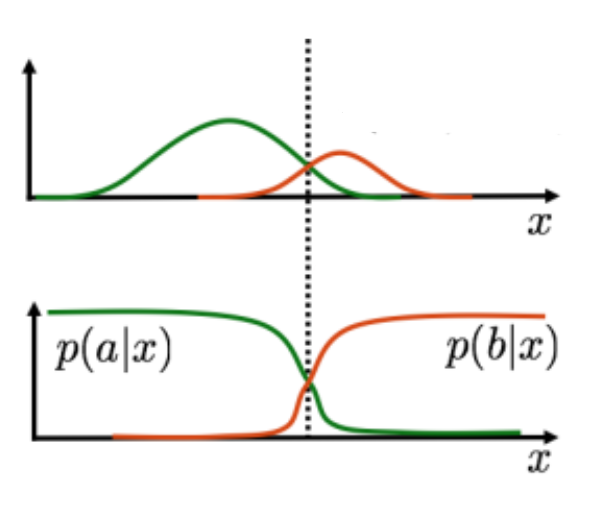
\includegraphics[width=0.5\linewidth]{boundaries.png}
    \end{center}
    \item When do we decide for class $C_1$ over $C_2$?\\
    We decide for $C_1$ when the posterior probability is higher.
    \[\frac{p(x|C_1)p(C_1)}{p(x)} > \frac{p(x|C_2)p(C_2)}{p(x)}\]
\end{itemize}
\end{solution}
\end{subtask}


%----------------------------------------------
\begin{subtask}[points=8,title=Decision Boundaries]
If both classes have equal prior probabilities $p(C_1) = p(C_2)$ and variances have the following relation  $\sigma_1 = 2\sigma_2$, derive the decision boundary $x^*$ analytically as a function of the two means $\mu_1$, $\mu_2$ and $\sigma_2$.

\begin{solution}
The decision boundary occurs where the posterior probabilities are equal: $p(C_1|x^*)=p(C_2|x^*)$. because the prior probabilities are equal, it simplifies to $p(x^*|C_1)=p(x^*|C_2)$. 
\begin{align*}
    p(x^*|C_1)&=p(x^*|C_2) \\ 
    \frac{1}{\sqrt{2\pi \sigma^2_1}}*\exp (-\frac{(x^*-\mu_1)^2}{2\sigma^2_1})&=\frac{1}{\sqrt{2\pi \sigma^2_2}}*\exp (-\frac{(x^*-\mu_2)^2}{2\sigma^2_2}) \\ 
    \text{Cancel out $\sqrt{2\pi}$ and use case $\sigma_1=2\sigma_2$}\\
    \frac{1}{2\sigma_2} \exp(-\frac{(x^*-\mu_1)^2}{2(2\sigma_2)^2})&=\frac{1}{\sigma_2}\exp (-\frac{(x^*-\mu_2)^2}{2 \sigma_2^2}) \,\,\,\, |*2\sigma_2 \\
    \exp (-\frac{(x^*-\mu_1)^2}{8\sigma_2^2}) &= 2 \exp (-\frac{(x^*-\mu_1)^2}{2\sigma_2^2}) \,\,\,\, | \ln \\ -\frac{(x^*-\mu_1)^2}{8\sigma_2^2} &= \ln(2) -\frac{(x^*-\mu_1)^2}{2\sigma_2^2}\,\,\,\, | * 8\sigma_2^2 \\
    -(x^*-\mu_1)^2&=8\sigma^2_2*\ln(2)-4(x^*-\mu_2)^2 \\
    -x^{*^2}-2x^*\mu_1+\mu_1^2&=8\sigma_2^2*\ln(2)-4(x^{*^2}-2x^*-\mu_2+\mu_2^2)\\
    3x^{*^2}+(2\mu_1-8\mu_2)x^*-(\mu_1^2+4\mu_2^2-8\sigma_2^2*ln(2)) &= 0\\
\end{align*}
To derive a formula to calculate $x^*$, we will use the quadratic formula
\begin{align*}
    f(\mu_1, \mu_2, \sigma_2)=x^*=\frac{-(2\mu_1-8\mu_2) \pm \sqrt{(2\mu_1-8\mu_2)^2-4*(3(-\mu_1+4\mu_2-8\sigma_2^2\ln(2)))}}{6}
\end{align*}
\end{solution}
\end{subtask}

% %----------------------------------------------
\newpage
\begin{subtask}[points=8,title=Different Misclassification Costs]

Assume $\mu_1 > 0$, 2$\mu_1 = 3\mu_2$, $\sigma_1=\sigma_2$ and $p(C_1) = p(C_2)$. If misclassifying sample $x \in C_2$ as class $C_1$ is six times more expensive than the opposite, how does the decision boundary change? Derive the boundary analytically in terms of $\mu_2$ and $\sigma_2$.
(There is no cost for correctly classifying samples.)
\begin{solution}
We know that The cost of misclassifying a instance of class $C_2$ is $6$ times higher as misclassifying a instance of class $C_1$. This leads to following ungleichung:
\[6\lambda*P(C_2|x)<\lambda*P(C_1|x)\]
There are also the correct classifications, but because those have no costs, they cancel out due to multiplication by 0.\\
Because of $P(C_1)=P(C_2)$ we can use the bayes rule in the following way:
\[6*p(x|C_2)*p(C_2)<p(x|C_1)*p(C_1) \,\,\,\, |:p(C_2); \text{ $C_1$ will also cancel out because they are equal}\]
\[6p(x|C_2)<p(x|C_1)\]

Now we substitute $p(x|C_i)$ witzh the gaussian distribution:

\[6*\frac{1}{\sqrt{2 \pi * \sigma^2}}*\exp (-\frac{(x-\mu_2)^2}{2*\sigma^2})<\frac{1}{\sqrt{2 \pi * \sigma^2}}*\exp (-\frac{(x-\mu_1)^2}{2*\sigma^2})\]

We use $\sigma$ for $\sigma_1$ and $\sigma_2$, because $\sigma_1=\sigma_2$. The starting fraction can cancel out and after applying $\ln$, we get:

\[\ln(6)-\frac{(x-\mu_2)^2}{2\sigma^2} <-\frac{(x-\mu_1)^2}{2\sigma^2} \,\,\,\, | * (-2\sigma^2)\]
\[(x-\mu_2)^2-2\sigma^2*\ln(6) > (x-\mu_1)^2\]

after expanding the sqared terms, we can cancel out $x^2$, and we will then re-formulate the ungleichung, so that $x$ is on one side.
\[2\mu_1x-2\mu_2x>\mu_1^2-\mu_2 ^2 + 2\sigma^2 \ln(6)\]
\[2(\mu_1x-\mu_2x)>\mu_1^2-\mu_2 ^2 + 2\sigma^2 \ln(6)\]

apply $\mu_1=\frac{3}{2}\mu_2$

\[2(\frac{3}{2}\mu_2-\mu_2)>(\frac{3}{2}\mu_2)^2-\mu^2_2 + 2\sigma^2\ln(6)\]
\[\mu_2x > \frac{5}{4}\mu^2_2+2\sigma^2\ln(6)\]

Because $\mu_1>0$ and $\mu_1=\frac{3}{2}\mu_2$, we know that $\mu_2>0, $ so we can devide by it
\[x > \frac{5}{4}\mu_2+\frac{2\sigma^2 \ln(6)}{\mu_2}\]

This means, we will decide for class $C_1$ if the inequality is true. Therefore we get following decision boundary $x^*$:

\[x^*=\frac{5}{4}\mu_2+\frac{2\sigma^2*\ln(6)}{\mu_2}\]

The boundary has moved because of the misclassification costs. Because it is more expensive to classify a data point from $C_2$ as $C_1$, the boundary is now at a position, where we need more evidence for $C_1$ to classify a data point as such. 

\end{solution}
\end{subtask}
\end{task}

\newpage

\begin{task}[points=11]{Risk Minimization}

Given is a classification problem of $N$ classes,
\[
C = \{C_1, C_2, \dots, C_N\}.
\]
We additionally introduce the option to assign a sample $x$ to none of the classes, which is denoted as $C_{\text{rej}}$. When the rejection risk is lower than the risk of assignment to each class $C_k \in C$, rejection can be a desirable action.

Let the true class of a sample $x$ be $C_k$ and the class it gets assigned to during classification be $C_j$. For any 
\[
k \in \{1,2,\dots,N\} \quad \text{and} \quad j \in \{1,2,\dots,N+1\},
\]
the loss is defined as
\[
\lambda_{jk} =
\begin{cases}
0, & \text{if } j = k, \\
l_{\text{reject}}, & \text{if } j = N+1, \\
l_{\text{misclassified}}, & \text{otherwise.}
\end{cases}
\]

\bigskip

\begin{subtask}[points=3]
 Derive the decision criterion that will give the minimum expected loss. \\
\textit{Hint:} 
\[
\text{classify}(x) \to \begin{cases}
C_k, & \text{if condition 1  \& condition 2 holds}, \\
C_{\text{rej}}, & \text{otherwise}
\end{cases}
\]
where the conditions are derived from comparing the expected risks.

\bigskip

\begin{solution}
The expected risk of assigning a sample $x$ to class $C_j$ is given by:

\[
R(C_j | x) = \sum_{k=1}^{N} \lambda_{jk} \cdot P(C_k | x)
\]


The risk of assigning to class $C_j$ whrere $j \le N$:
\[
R(C_j | x ) = \lambda_{\text{misclassified}} \cdot (1 - P(C_j | x))
\]

The risk of rejection:
\[
R(C_j | x ) = \lambda_{\text{reject}}
\]

The decision criterion is that we want to choose an action with the lowest risk.
So we assign to class $C_j$ only if:
\[
R(C_j | x ) \le R(C_{\text{rej}} | x) \Rightarrow \lambda_{\text{misclassified}} \cdot (1 - P(C_j | x)) < \lambda_{\text{reject}} \Rightarrow P(C_j | x ) > 1 - \frac{\lambda_\text{reject}}{\lambda_\text{misclassified}}
\]

Also, among all classes, we want the one with the maximum posterior:
\[
j = \arg \max_k P(C_k | x)
\]

The final decision rule is:
\[
\text{classify}(x) \to \begin{cases}
C_k, & {P(C_k | x ) = max_j P(C_j | x) \text{ \& }  P(C_k | x ) > 1 - \frac{\lambda_\text{reject}}{\lambda_\text{misclassified}}}, \\
C_{\text{rej}}, & \text{otherwise}
\end{cases}
\]

\end{solution}
\end{subtask}

\vspace{2em}

\begin{subtask}[points=2]
What happens if $l_{\text{reject}} = 0$?

\begin{solution}
If $l_{\text{reject}} = 0$, then rejecting a classification has no penalty, which means that it is risk-free.

If we take a look at the decision rule from task 6a
\[
\text{classify}(x) \to \begin{cases}
C_k, & {P(C_k | x ) = max_j P(C_j | x) \text{ \& }  P(C_k | x ) > 1 - \frac{\lambda_\text{reject}}{\lambda_\text{misclassified}}}, \\
C_{\text{rej}}, & \text{otherwise}
\end{cases}
\]

with substituting $\lambda_{\text{reject}} = 0$:
\[
R(C_k ] x ) > 1 - \frac{0}{\lambda_\text{misclassified}} = 1
\]

This condition becomes never true becuase probabilities are always $\leq$ 1

The result is that if $l_{\text{reject}} = 0$, the classifier will always reject every input, because any classififcation has non-zero expected loss, while rejection has zero loss.

\end{solution} 
\end{subtask}

\vspace{2em}
\begin{subtask}[points=1]

 What happens if $l_{\text{reject}} > l_{\text{misclassified}}$? 

\begin{solution}
If $l_{\lambda{\text{reject}}} > l_{\lambda{\text{misclassified}}}$, we can convert it to:
\[
\frac{\lambda_\text{reject}}{\lambda_\text{misclassified}} > 1
\]

Then the threshold in the decision rule becomes:
\[
P(C_k | x) > 1 - \frac{\lambda_\text{reject}}{\lambda_\text{misclassified}} < 0
\]

Since $1 - \frac{\lambda_\text{reject}}{\lambda_\text{misclassified}} < 0$, the condition will always be satisfied for any valid probability $P(C_k | x) \in [0, 1]$.

This means that rejection will never happen, even if the classifier is very uncertain, that value will always be greater than a negative threshold.
The classifier will always aaging the most probable class.

\end{solution}
\end{subtask}
\newpage
\begin{subtask}[points=5]
In risk minimization, the rewards/costs assigned to different decision options (such as correct classification, rejection, or misclassification) play a key role in determining the algorithm’s behavior.

Who should determine these rewards/costs, which factors should be considered, and how? Propose a process for determining the adequate rewards/costs in a loan approval algorithm.

\begin{solution}
In risk minimization, the rewards and costs assigned to different decision outcomes—such as correct classification, misclassification, or rejection—fundamentally shape how a model behaves.

\textbf{Who Should Determine the Rewards/Costs?}

The assignment of rewards and costs should not be left solely to technical teams. It requires input from a group, including:
\begin{itemize}
    \item Domain experts – to provide insight into the real-world impact of decisions.
    \item Risk and compliance officers – to ensure decisions align with regulations and avoid unfair outcomes.
    \item Data scientists and ML engineers – to translate these qualitative inputs into quantitative values used in model training and evaluation.
    \item Business stakeholders – to align cost/reward assignments with strategic goals and acceptable risk thresholds.
\end{itemize}

\textbf{Factors to Consider}

When assigning costs and rewards in classification systems, the following factors should be consider:

\begin{itemize}
    \item Severity of misclassification: Some misclassifications have much higher stakes than others.
    \item Uncertainty in model predictions: The model may prefer low-confidence predictions if rejection incurs lower loss than a potential mistake.
    \item Cost of rejection: Rejection may involve handing over decisions to humans, which could have operational costs or delay consequences.
    \item Long-term consequences: Consider reputation damage, user trust, or future legal risks associated with systematic bias or errors.
\end{itemize}

\textbf{How Should the Costs Be Determined?}

\begin{enumerate}
    \item Define all possible outcomes: True positive, false positive, true negative, false negative, and rejection.
    \item Estimate the real-world impact (financial, social, or legal) for each outcome.
    \item Translate these impacts into loss values that reflect relative severity.
    \item Test and validate using historical data, evaluating performance and fairness.
    \item Refine and adjust periodically as societal, legal, or business factors evolve.
\end{enumerate}

\textbf{Process for Determining Adequate Rewards/Costs in a Loan Approval Algorithm}

For a loan approval system, the process can be made specific as follows:
\begin{enumerate}
    \item Enumerate outcomes
    \begin{itemize}
        \item Approve a good applicant (true positive).
        \item Approve a risky applicant who defaults (false positive).
        \item Reject a bad applicant (true negative).
        \item Reject a good applicant (false negative).
        \item Reject due to uncertainty (rejection option).
    \end{itemize}

    \item Quantify impacts \begin{itemize}
        \item Calculate expected profit from repaid loans and expected losses from defaults.
        \item Estimate the opportunity costs of rejecting reliable applicants.
        \item Define operational costs for rejected applications (e.g. manual review or lost customers).
    \end{itemize}

    \item Assign cost values
    \begin{itemize}
        \item \( l_{\text{correct}} = 0 \)
        \item \( l_{\text{misclassified}} \): Potential financial loss from a default.
        \item \( l_{\text{reject}} \): Cost of manual review or user dissatisfaction.
    \end{itemize}

    \item Simulate decisions
    \begin{itemize}
        \item Apply the model to historical loan data.
        \item Adjust costs based on observed default rates, approval accuracy, and business outcomes.
    \end{itemize}

    \item Review
    \begin{itemize}
        \item Ensure that the cost structure reflects business risk tolerance, fairness expectations, and compliance needs.
        \item Update regularly based on market trends and regulatory updates.
    \end{itemize}
\end{enumerate}

\end{solution}
\end{subtask}
\end{task}

\

\end{document}